\def\erf{\mathord{\rm erf}}
\def\q#1{q_{\mbox{\scriptsize #1}}}

\section{Motivation} % (fold)

Flooding resulting from excessive precipitaion and surface runoff is a principle cause of significant damage, loss of property, and human suffering throughout the world.  During the GEMT 2010 study group at the Centre de Recerca Matem�tica(UAB) in Barcelona our team was given the task of determining a mathematical model to optimize gate operation along the Ebro River in Spain.   We designed a simple model in which we assumed that the flood wave would maintain its original shape as it propagated downstream.  This simplified model of the situation allowed us to look more closely at the mathematics involved in river flooding and gain some insight on a basic strategy for regulating the flood gates.  In addition to deriving this model for gate regulation we also investigated the costs associated to the situation when $\q{f} > \q{max}$, i.e. the situation where flooding cannot be avoided.  In this situation it is important to minimize the costs in terms of human suffering and property damage.  We investigate in this paper two methods for approaching the situation where flooding cannot be avoided, there are two methods to consider in this case, Strategy A: opening the gates when $\q{f}$ is achieved, or Strategy B: opening the gates when $\q{max}$ is achieved, this paper will discuss the analysis of both strategies in detail.  Finally at the conclusion of our analysis we will state some future problems that might be taken up by our group or other researchers with an interest in this problem.  
% (end)

\section{First Simple Model} % (fold)

First we will discuss a simple control strategy:
\begin{quote}
	Given a set point $\q{f}$, open the gates completely when the discharge reaches this threshold.
\end{quote}

As a simple first approximation, we ignored the geometry of the river bed and assumed that the flood wave would maintain its shape as it propagated down the river.
We will also assume the height of the river at a given point depends only on the discharge at this point by a increasing function.
In this way we could use height and discharge interchangeably.

Given that opening a gate to a floodplain can reduce the flood by a given volume $W$, we look for the set point $\q{f}$ to
open and close the gate in order to reduce the flood by this area optimally.
Mathematically speaking, if we define the discharge of a flood wave at the gate point as $q(t)$ and
pick a reference instant $t_{0}$ before the start of the flood and define for all $0<y\leq\q{i}$
\begin{equation}
V(y)=\int_{t_{0}}^{t_{1}}\left[q(t)-y\right]_{+}\, dt\leq W,
\end{equation}
where $\left[x\right]_{+}=\max\{x,0\}$ and $\q{i}$ is the forecast maximum discharge
(which is taken at instant $t=t_m$).
This expression could be
written on the time interval defined by the condition $q(a)=q(b)=\q{f}$ and $q(t) > \q{f}$ for $t\in(a,b)$
using an iterated integral as
\[
V(y)=
\int_{a}^{b}\left(\int_{y}^{q(t)}dq\right)dt.
\]
By inverting the order of the integration, we get
\begin{equation}
V(y)=
\int_{y}^{\q{i}}\left(\int_{t_{-}(q)}^{t_{+}(q)}dt\right)dq=
\int_{y}^{\q{i}}(t_{+}(q)-t_{-}(q))\, dq,	
\end{equation}
where $t_{-}(q)$
(respectively $t_{+}(q)$) is the unique $t<t_{m}$ (respectively
$t>t_{m}$) with $q(t)=q$. Since $V'(y)=t_{-}(y)-t_{+}(y)\leq0$,
$V(y)$ is decreasing with $V(\q{i})=0$ and it is easy to find the
unique point $\q{f}$ such that $V(\q{f})=W$ by numerical integration
followed by bisection or inverse interpolation.




\subsection{An Example}
\marginpar{\scriptsize Numerical experiment instead?}
In the problem we are given that the initial profile of the floodwave is a Gaussian:
\begin{equation}
q(t)=q_p \exp(-\frac{t^2}{2t_b^2})
\end{equation}
where $q_p$ is the peak of the flood, and $t_b$ is the duration of the flood. So in this case
\begin{align}
V(t)&=q_p \int_{-\infty}^t \exp(-\frac{s^2}{2t_b^2}) ds \notag \\
 &=q_p t_b \sqrt{\frac{\pi}{2}} \erf(\frac{t}{t_b\sqrt{2}})
\end{align}
giving us that 
\begin{equation}
t(V)=t_b\sqrt{2}\erf^{-1}(\frac{V}{q_p t_b} \sqrt{\frac{2}{\pi}})
\end{equation}
and
\begin{equation}
q(V)=q(t(V))=q_p \exp \bigl( -[\erf^{-1}(\frac{V}{q_p t_b} \sqrt{\frac{2}{\pi}})]^2 \bigr) 
\end{equation}

Here's a diagram:

\marginpar{\scriptsize Where are the figures?}
\begin{figure} \centering
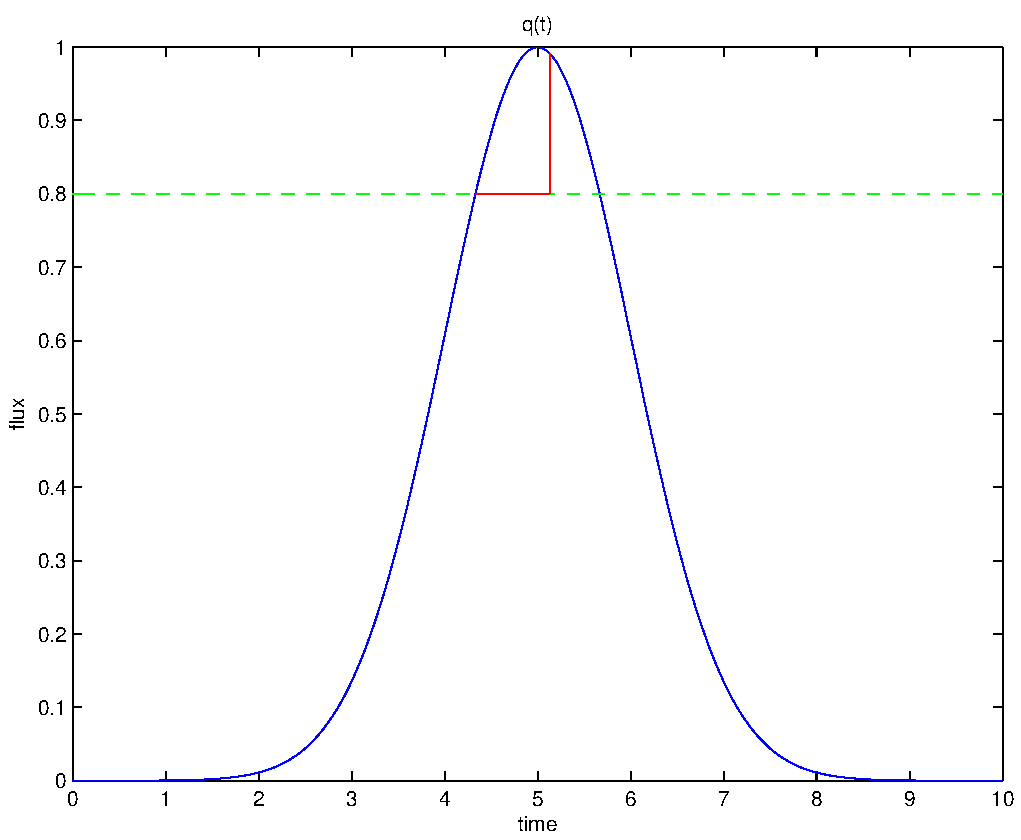
\includegraphics[width=8cm]{fig1}
\caption{Flux versus time for simple Gaussian Peak}
\label{1}
\end{figure}
% (end)

\section{Heavy Flooding} % (fold)

However, when the flooding is particularly heavy, the capacity of the floodplains maybe insufficient. In this case, even when the peak of the flood is reduced by $W$, it is still higher than $\q{max}$ the levee height, causing floods. In this situation we have two options for controlling the gates, the first strategy is that the gates are opened as soon as the water level reaches $\q{max}$ and the resevoir is filled to capacity, hence reducing the front of the floodwave. This then gives us more time to deal with the flood, e.g. preparing to open more gates downstream. 

Here's a diagram:

\begin{figure} \centering
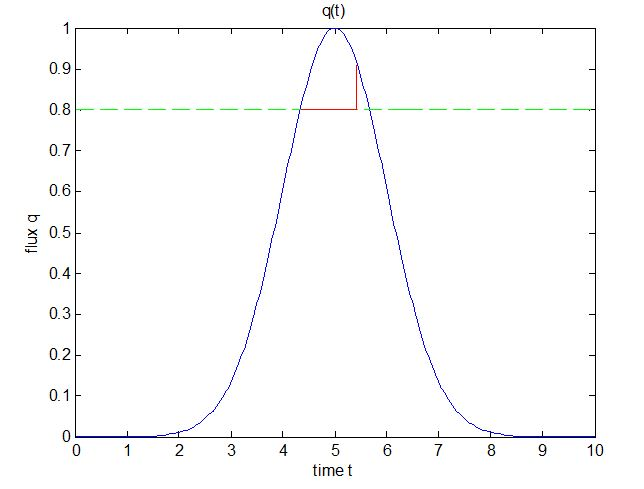
\includegraphics[width=8cm]{fig2}
\caption{Flux versus time for a peak where flooding is inevitable}
\label{1bis}
\end{figure}

In the case of flows with multiple flood waves it is always ideal to open the gates at $\q{max}$ instead of $\q{f}$ as it allows some capacity of the floodplain to be reserved for later flood waves. Thus when we have multiple flood waves we will never open the gates before $q = \q{max}$.  

Here are a few diagrams of the situation involving multiple waves:

\begin{figure} \centering
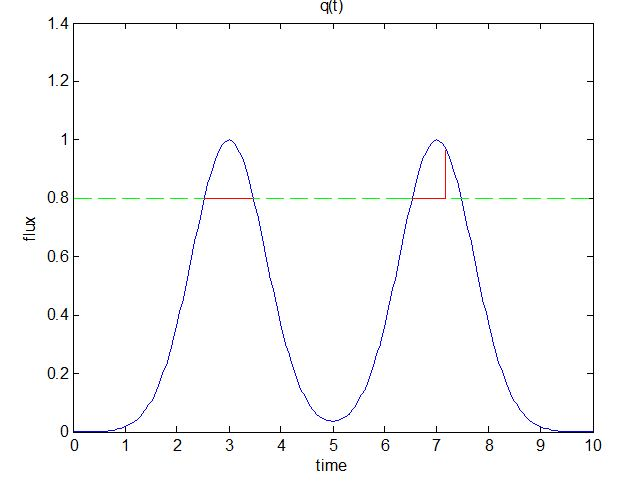
\includegraphics[width=8cm]{fig5}
\caption{Opening the gate at $\q{max}$ allows maximum remaining capcity for the second flood wave.}
\label{2}
\end{figure}

The next diagram illustrates a case where we can do even better:

\begin{figure} \centering
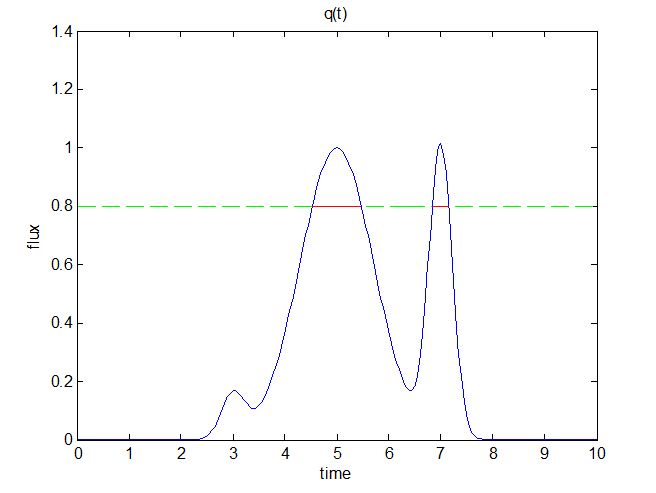
\includegraphics[width=8cm]{fig7}
\caption{Opening the gate at $\q{max}$ allows us to prevent flooding entirely in this case.}
\label{3}
\end{figure}
% (end)

\section{Cost modelling of the two main strategies in a flooding} % (fold)

\subsection*{Main problem: there are two possible strategies}
We have two possible strategies to follow when scenario $\q{max}<\q{f}$ occurs and thus we can not avoid the flood: we can either choose to open the gate when the flow $q$ achives $\q{max}$ or open it when $\q{f}$ is achived. Each strategy has its advantages: 
\begin{itemize}
\item On the one hand, if we open the gate at $\q{max}$, we are going to be delaying the flood as much as we can, but when it arribes, the effects will be quite important. 
\item On the other hand, if we wait to open the gates until $q$ achieves $\q{f}$, the flood will arrive sooner, but its effects will be reduced, because the intensity of the flow is going to be lower.
\end{itemize}

\subsection*{Designing a cost function: a possible solution}
Thus, we want to design a cost function in order to measure the ``cost'' of each strategy. This cost function will take on account the number of affected people depending on the heigh of the water in the flood and also the time that the strategy is are able to delay it. The cost function that we are going to consider is defined as equation \ref{cost} shows. The cost that we are assuming from an initial time $t_i$ to a certain time $t$ is given by:
\begin{equation}
C(t)=\int_{t_i}^{t}\frac{\rho(h(q(t)))}{t}dt,
\label{cost}
\end{equation}
where $\rho$ is the density of population that lives below a certain heigh $h$ (where the heigh depends on $q$, both $q$ and $h$ known). We have divided the density by $t$ in order to ``decrease the cost'' when increasing the time, since we want to minimize the effects of the flood but also give time to the population to leave the most affected zones. If we want to give more importance to the delay of the flood we can change the modelling cost and use some other $t^r$, $r>1$.

\subsection*{Finding the strategy that minimizes the cost function}
We want then to compute the cost function for each one of the two main strategies to follow in a flooding scenario. Hence, the most valid strategy will be the one that gives the minimum final cost at the ending time $t_f$.

\subsubsection*{Strategy A: opening the gates when $\q{f}$ is achieved}
\begin{figure} \centering
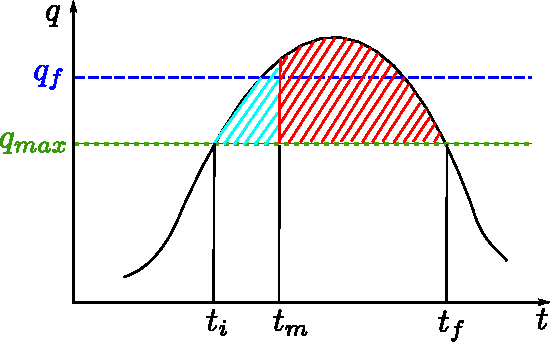
\includegraphics[width=8cm]{basicA}
\caption{Flow diagram for strategy A}
\label{A}
\end{figure}
Figure \ref{A} shows that with strategy A we are going to be able to eliminate the flow marked in light blue. The dangerous flow that we are not going to be able to stop and that is going to be penalized by the cost function is marked in red. To be able to compute the cost function, we need the population density of the affected zone. However, we can easily find an upper bound for the cost of this strategy:
\begin{eqnarray*}
C(t_f)&=&\int_{t_i}^{t_f}\frac{\rho(h(q(t)))}{t}dt\overset{q(t)\leq \q{f}(t)\ \forall t}{\leq} \int_{t_i}^{t_f}\frac{\rho(h(\q{f}(t)))}{t}dt\\
&=&\int_{t_i}^{t_f}\frac{\rho_{\q{f}}}{t}dt=\rho_q\cdot\ln(\frac{t_f}{t_i}),
\end{eqnarray*}
where we have denoted by ${\rho_{\q{f}}}$ the density of population that lives below $h(\q{f})$.

Thus, we can bound
\marginpar{\tiny this may be useful if we could compare it with B... but we are not able to do so... we need $\rho$ in order to be able to say something)}
the cost of strategy A as
\begin{equation}
C_A\leq\rho_q\cdot\ln(\frac{t_f}{t_i}),
\label{CA}
\end{equation} 
where $\rho_{\q{f}},\ t_i \text{ and } t_f$ are all known.

\subsubsection*{Strategy B: opening the gates when $\q{max}$ is achieved}
\begin{figure} \centering
\includegraphics[width=8cm]{basicB}
\caption{Flow diagram for strategy B}
\label{B}
\end{figure}
With strategy B we find that despite reaching higher flow values, the time in which $\q{max}$ is achieved is delayed, and thus there are no ``human'' costs until a bigger time than the one used in strategy A. However, we are just able to delay the flow into a known time $t_m$, where the auxiliar area is full and we can not take more water from the river. Thus, the cost of strategy B is
\begin{eqnarray*}
C(t_f)=\int_{t_i}^{t_f}\frac{\rho(h(q(t)))}{t}dt=\int_{t_m}^{t_f}\frac{\rho(h(q(t)))}{t}dt,
\end{eqnarray*}
where we must recall that all the data required in the integral is known, and thus, in a particular case it is straight forward to compute the cost.

Hence,
\begin{equation}
C_B=\int_{t_m}^{t_f}\frac{\rho(h(q(t)))}{t}dt,
\label{costB}
\end{equation}
and then depending on the scenario that is placed we can compute both $C_A$ and $C_B$ and have a reference of which one of the strategies will bring up more advantages.
% (end)

\section{Conclusion and Further Work} % (fold)

In this paper we have stated an algorithm for determining the opening and closing times of a single flood gate.  In addition we have studied how cost functions can be used to minimize damage and hardship caused by flooding in highly populated areas along the Ebro River.

We propose that in future research studies the case of gate control is considered more closely, perhaps in conjunction with the idea of minimizing costs in the case that flooding cannot be avoided.  The most important extension of our ideas is to work with multiple gates and multiple flood waves.  This case will be more complex but also will more closely impact actual implementation of gate control along the Ebro River.  By assigning a cost to the flooding of particular floodplains it will be possible to obtain the minimum amount of damage in the case that we cannot prevent a flood with the gate control scheme.  
% (end)